\documentclass[a4paper]{report}
\usepackage[english]{babel}
\usepackage{amsmath}
\usepackage{graphicx}
\usepackage{subcaption}
\usepackage{placeins}

\author{Maarten de Jonge \\
        Inge Becht}
\date{\today}
\title{Various Models and Simulations}

\begin{document}
\maketitle

\chapter{Simulating a forest fire with a cellular automaton}
\label{cha:ff}

\section{Implementation} 
\label{sec:ff_impl}

The simulation is implemented as a cellular automaton using the following simple
rules:
\begin{enumerate}
    \item A cell can be empty, vegetated, burning, or burnt.
    \item A vegetated cell will become burning if one of its neighbours is
          burning.
    \item A burning cell will become burnt.
\end{enumerate}
where ``neighbour'' is defined as being in the 8-cell Moore-neighbourhood of a
cell and rules 2 and 3 govern the transition from one moment in time to the
next.

The playing field gets initialised with a certain vegetation density, which
gives the probability of each individual cell starting out in the vegetated
state (a cell starts out vegetated if $Q <= D$ where $D$ is the vegetation
density and $Q$ is a random float between 0 and 1). The entire bottom row will
be set on fire initially (regardless of the content of the cells). The
simulation runs until there are no more burning cells.

\begin{figure}[htbp]
    \centering
    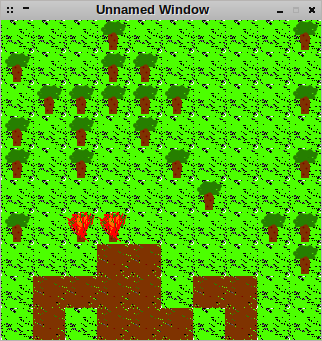
\includegraphics[width=0.7\textwidth]{./sdl.png}
    \caption{a visualisation of the forestfire automaton}
    \label{fig:sdl}
\end{figure}

Just for fun, a visualisation has been made using the SDL library (figure
\ref{fig:sdl}).

% section ff_impl (end)

\section{Experimentation} 
\label{sec:ff_exp}

After each run of the simulation, the following data was collected:
\begin{itemize}
    \item Whether the other side of the field (the top-side, since the fire
        starts at the bottom) had been reached.
    \item How many steps it took to the other side (0 if it wasn't reached).
    \item The percentage of vegetation that was burnt.
\end{itemize}

The simulation has been run 250 times with the parameter tuples $(FieldSize,
Density)$, where $FieldSize \in \{10, 15, 20, 25, 30, 35\}$ and \\
$Density \in \{0.05, 0.1, 0.2, 0.3, 0.4, 0.5, 0.6, 0.7, 0.8, 0.9\}$, leading to
$6 \times 10$ trials being run 250 times each. The field
was chosen to be square, leading to a $FieldSize \times FieldSize$ sized field.

The results were plotted as heatmaps because of the large amount of overlapping
points, and are shown in figures \ref{fig:reached}, \ref{fig:steps} and
\ref{fig:burnt}.

\begin{figure}[htbp]
    \centering
    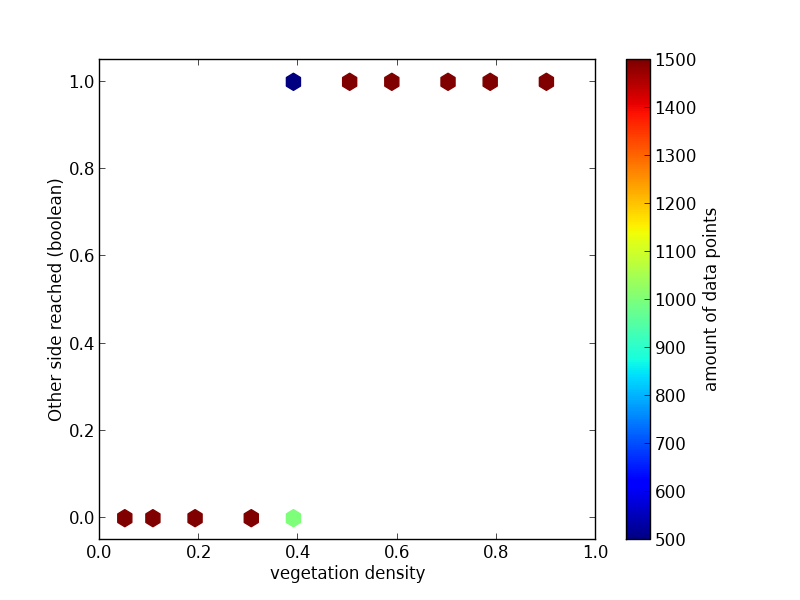
\includegraphics[width=0.7\textwidth]{./density_vs_reached.png}
    \caption{A boolean plot showing whether the other side was reached (1 =
             reached, 0 = not reached)}
    \label{fig:reached}
\end{figure}

\begin{figure}[htbp]
    \centering
    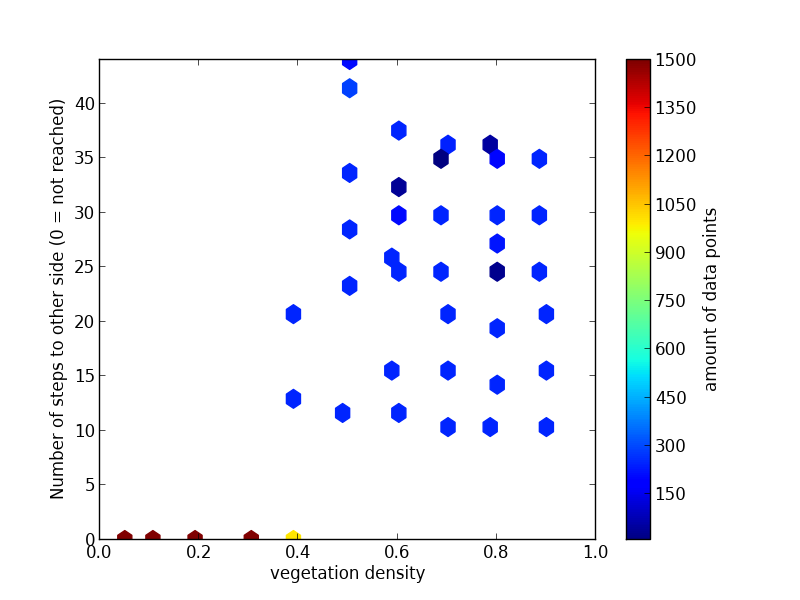
\includegraphics[width=0.7\textwidth]{./density_vs_steps.png}
    \caption{Number of steps to reach the other side as function of the density.
             A value of 0 means the other side wasn't reached.}
    \label{fig:steps}
\end{figure}

\begin{figure}[htbp]
    \centering
    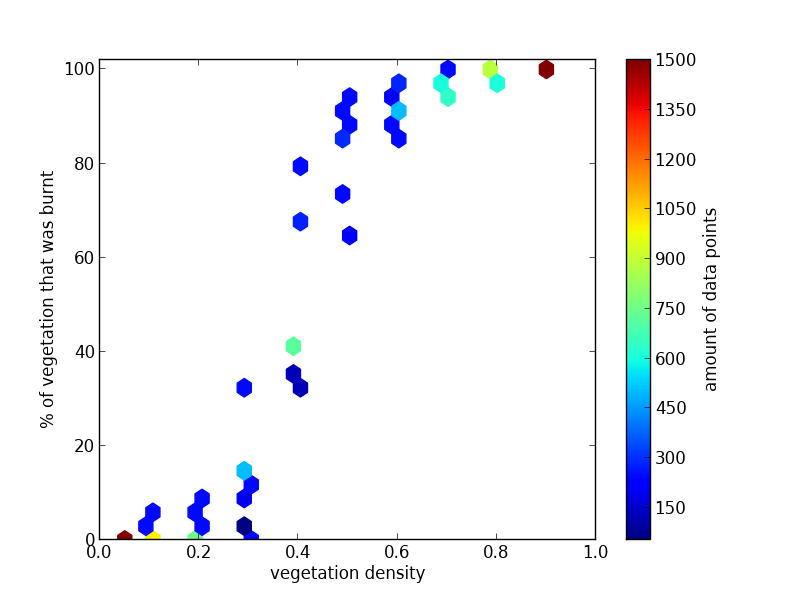
\includegraphics[width=0.7\textwidth]{./density_vs_burnt.png}
    \caption{Percentage of burnt trees as function of the density.}
    \label{fig:burnt}
\end{figure}

\begin{figure}[htbp]
    \centering
    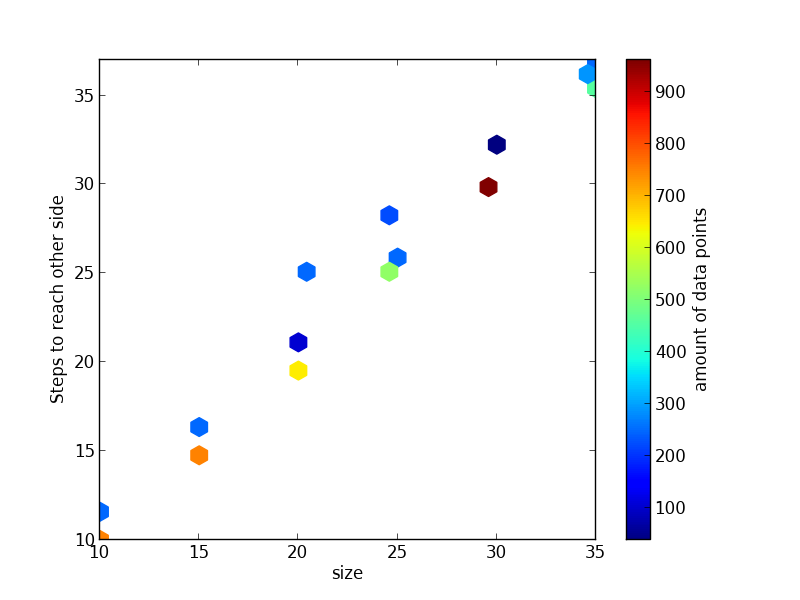
\includegraphics[width=0.7\textwidth]{./size_vs_steps.png}
    \caption{Field size vs steps to other side, restricted to densities of [0.6,
    \label{fig:size}
0.9]}
\end{figure}


% section ff_exp (end)

\section{Results} 
\label{sec:ff_results}

Looking at the reaching of the other side, there's clearly a hard threshold
around a density of $0.4$. Below $0.4$ none of trials reach the other side, while
above it 100\% of the trials reach it. At $0.4$ it varies, with a majority of
trials not reaching the other side.

The steps required to reach the other side looks to be roughly evenly divided
between 10 and 40 steps at densities of $0.6$ and up, with a slightly higher
boundary (45) at a density of $0.5$. Keeping in mind that the simulation was run
at various different sizes for the field, it is reasonable to suspect that this
has an influence on the required steps to reach the other side. To be sure of
this, the fieldsize has been plotted against the required steps, filtered for
densities from 0.6 to 0.9 (figure \ref{fig:size}). This shows that in general,
it takes about $n$ steps for the fire to get to the other side of an $n \times
n$ field, sometimes slightly more.

The percentage of burnt trees increases with a roughly S-shaped curve, with the
percentage quickly increasing with the middle densities, and more slowly at the
extremes, culminating at a (practically) 100\% burn rate at a density of $0.9$.

% section ff_results (end)

\section{Conclusion} 
\label{sec:ff_conc}

The act of fire reaching the other side displays a threshold effect around a
density of $0.4$ - $0.5$. A density of $0.5$ is enough for the fire to reach the
other side in every trial, and from $0.6$ on it is generally reached in the
minimum possible amount of steps.

The percentage of burnt trees acts a bit more sigmoid-like, displaying an
S-shaped curve from 0\% to 100\%.

Thus if you want to burn down a forest and get the fire to the other side, the
density of the forest doesn't matter as long it's over $0.5$. However if you
hate nature and want to burn down as much forest as possible, pick the forest
with the highest density. Conversely, if you're planning to construct a new
forest and are scared of potential evildoers, keeping the vegetation density
below $0.4$ will generally prevent a fire from going all the way across your
forest.

% section ff_conc (end)

% chapter ff (end)

\chapter{A grid-simulation of the spread of malaria}
\label{cha:malaria}

In this grid-simulation a representation is made of how malaria can spread
throughout a small population of humans and how well it can flourish
depending on human and mosquito density. 

The spread of malaria is quite complex and had to be simplified to be modeled as
a grid-simulation, hence the following assumptions were made:

\begin{itemize}
    \item A human can be susceptible, infected, immune or dead. None of the states are
        permanent except for death.
    \item A mosquito can be susceptible, infected or dead. 
    \item Mosquitoes can move to neighbouring cells. All mosquitoes make a
        random move if possible, and else stay where they are.
    \item Humans are stoic.
    \item Only one mosquito can occupy a cell at a time iteration, but both a
        human and a mosquito can be in the same cell.
    \item Both humans and mosquitoes can die and for every died person or
        mosquito a new uninfected one is born.
    \item Humans will spawn next to an already existing human, and the same for
        mosquitoes (creating clusters, as is shown in figure \ref{fig:clustering}).
    \item If a susceptible mosquito bites an infected human, it changes to the
        infected state. If an infected mosquito bites an uninfected human it
        changes the human to the infected state. All other cases won't change
        the states. Biting only happens when a mosquito and a human are on the
        same cell.
    \item In the first state each cell contains one or no elements. So
    if a simulation has dimension $n \times m$, than the amount of elments can
    at max be $n \times m$. Figure \ref{ascii} gives a visual representation of
    such a starting grid to give a better idea of how it looks.
    \item Each time iretation the mosquitoes move one space, people change state
        (new ones spawn)
        and people can get bitten.
    \item The grid is not a torus but a bounded rectangle. This because of
        implementation simplicitity, but seems more like real life as well.
\end{itemize}


\begin{figure}[htbp]
    \centering
    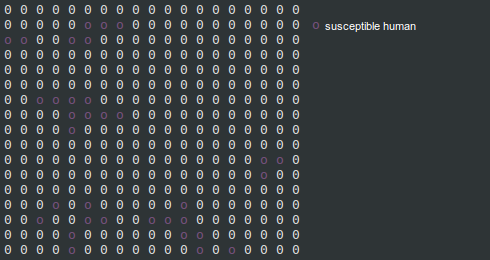
\includegraphics[width=1\textwidth]{population_clusters.png}
    \caption{A visualtion of cluster forming (around 300 runs)}
    \label{fig:clustering}
\end{figure}

\begin{figure}[htbp]
    \centering
    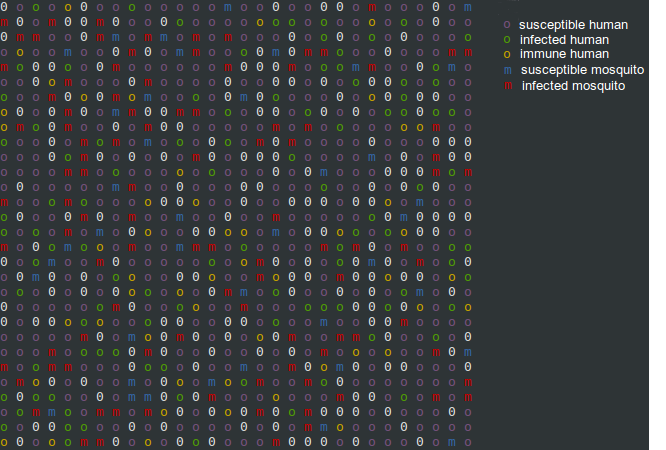
\includegraphics[width=1\textwidth]{malaria_ascii.png}
    \caption{A visualtion of the initial state of the grid simulation. }
    \label{fig:ascii}
\end{figure}

\section{Experimentation} 
For the following experiments a $30 \times 30$ grid was used. Every simulation ran exactly
500 times, or until no longer any infected humans or mosquitoes were present on
the board (i.e. when  malaria became extinct). If more than 500 runs
were used this is stated so explicitly in the results.
Because every board instance is random, each choice of combination density ran
twenty times so that the random factor would be excluded as much as possible
from the output (while still making the execution times manageable).

For these experimentations the rates from table \ref{tab:rates} were used in all
cases, if not explicitly told otherwhise. These rates are not the basis of the
experiments, but are just used to initialise the world in some manner (that is
plausible). The real experiment lies in the rates of density for both
humans and mosquitoes, as well as the starting percentage of susceptible
humans and mosquitoes and their e fect on the spread of malaria. A good
explanation  is 
tried to be given for the cohesion between population density and how well maleria can live in these conditions.
When experimentations do deviate from the rates of table \ref{tab:rates} this is
done with the purpose of showing the cohesion between these rates and the
densities..

\begin{table}
\centering
\begin{tabular}{|l|l|r|}
        \hline
        variable&for&rate\\
        \hline
        mortality rate&susceptible humans &0.003\\
        mortality rate&infected humans&0.03\\
        mortality rate&immune humans&0.003\\
        mortality rate&susceptible mosquitoes&0.045\\
        mortality rate&infected mosquitoes&0.045\\
        turning susceptible&immune humans& 0.06\\
        hungry&infected mosquito  & 0.3\\
        hungry&uninfected mosquito& 0.3\\
        infectionrate&infected mosquito& 1\\
        \hline
\end{tabular}
\caption{Rates used for experimentations }
\label{tab:rates}
\end{table}

\section{Results}

\subsection{Varying densities} 
Intuitively the most important criterium for the sustainability of malaria would
seem to be the amount of humans on the grid that would be able to catch the
disease. The more humans, the more uninfected mosquitoes might possibly get
infected as well and the longer the disease will probably survive. Figure
\ref{fig:var_human} shows the statistics. The
experimentation was conducted with 450 mosquitoes (half of the grid) from which
396 were susceptible.  For every run the rate of humans (in relation to total
grid size) was 0.1, 0.2, 0.3, 0.4
and 0.5 (note that 0.5 is the max as the amount of mosquitoes is 450, or 0.5, as
well). The amount of susceptible humans is 0.2 of the total amount of humans.
Figure \ref{fig:var_human} shows that malaria in a smaller population doesn't
flourish so well. In case of 0.1 ratio of human population malaria dies out
after around 350 iterations. In case of 0.2, the amount of infected mosquitoes
is quite low and seems to go down still after 500 iterations.
 In the case of the 0.4 and 0.5 ratio, a stabilisaion point seems to
develop, with the most infected mosquito at a time in case of a 1 to 1 ratio of
mosquitoes and humans. Figure \ref{fig:var_human_1500} shows the development towards 1500
iterations, for both 360 en 450 humans. Both having a stabilised infected
mosquito population of around 0.4 and 0.5 of the total mosquito population
respectively. The rate of infected humans stabilises around 0.1 and  0.2,
making the case of a 1:1 ratio (450 mosquitoes and 450 humans) the best
combination for spreading malaria in these given cases.

An experiment with more mosquitoes than humans is conducted as well. In figure
\ref{fig:more_mosquitoes}
the effect of having 630 mosquitoes next to 270 humans is shown with a human
susceptibility rate of 0.8 and those of mosquitoes of 0.2. The amount
of infected mosquitoes after the $500$th iteration lays around 246, or a rate
of 0.39 of the total mosquito population. The amount of infected humans
is about 0.33 of the total amount of humans, performing about as good as the
1:1 ratio. the ratio of infected humans is higher but because the lower
population it is less nuanced as in the previous case and can be neglected

Table \ref{tab:rates_density} shows all results in table format.

\begin{figure}[htbp]
    \centering
    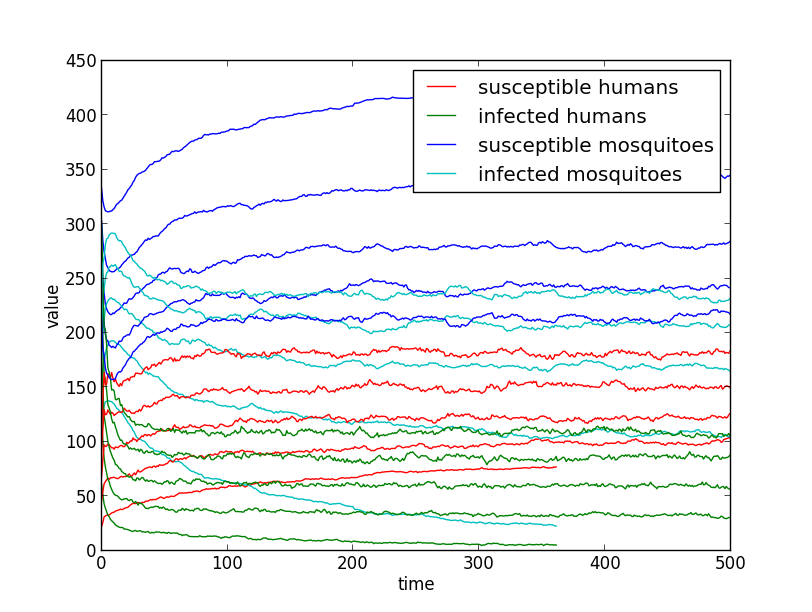
\includegraphics[width=0.9\textwidth]{var_human_density_02_05_08_SECOND.png}
    \caption{The result of varying human density between 90 humans and 450 humans.}
    \label{fig:var_human}
\end{figure}

%TODO: 1500 run for both 0.4 and 0.5 humans

\begin{figure}[htbp]
    \centering
    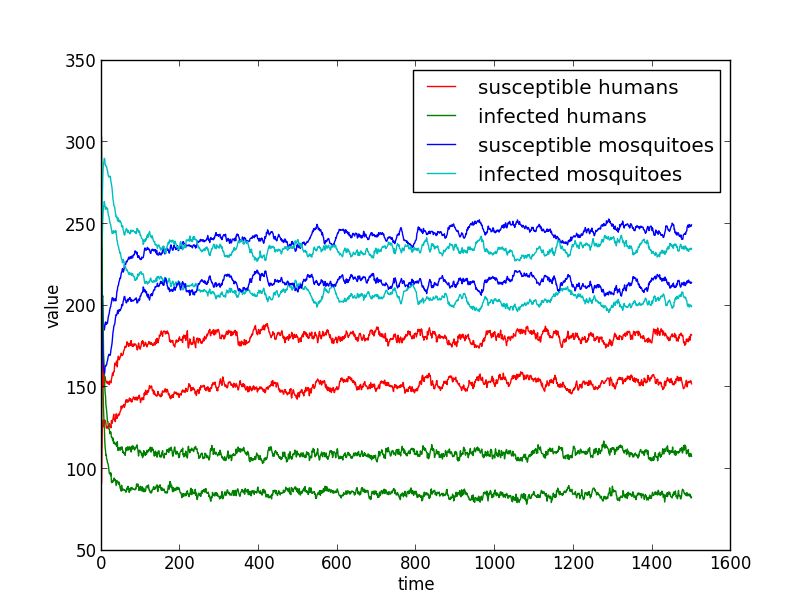
\includegraphics[width=0.9\textwidth]{var_human_1500_SECOND.png}
    \caption{Extended towards 1500 iterations for population of 360 and 450
    humans}
    \label{fig:var_human_1500}
\end{figure}

%TODO: Show 0.6 humans and variety of mosquitoes?

\begin{figure}[htbp]
    \centering
    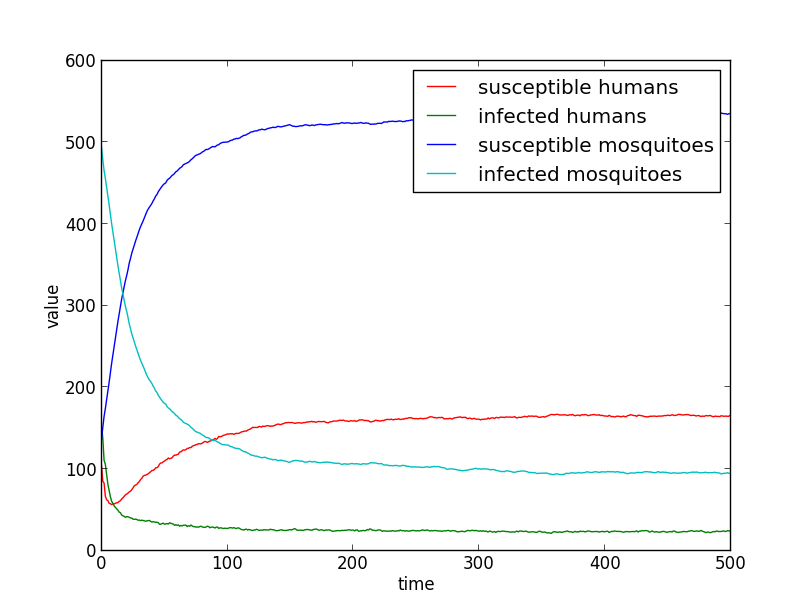
\includegraphics[width=0.9\textwidth]{03_08_07_02.png}
    \caption{In case of a rate of 0.7 mosquitoes against a rate of 0.3 humans
    }
    \label{fig:more_mosquitoes}
\end{figure}


\FloatBarrier
\begin{table}
\centering
\scalebox{0.8}{
\begin{tabular}{|r|r|r|r|r|r|}
        \hline
        human dens.&human susc.&mosquito dens.&mosquito
        susc.&inf. humans 500 it.& inf. mosquito 500 it. \\
        %a&a&a&a&a&a\\
        \hline
        0.1&0.8&0.5&0.2&0&0\\
        0.2&0.8&0.5&0.2&0.07&0.23\\
        0.3&0.8&0.5&0.2&0.12&0.38 \\
        0.4&0.8&0.5&0.2&0.15&0.45\\
        0.5&0.8&0.5&0.2&0.23&0.51\\
        0.3&0.8&0.7&0.2&0.33&0.39\\
        \hline
\end{tabular}
}
\caption{Rates used for density experimentation}
\label{tab:rates_density}
\end{table}
\FloatBarrier

\subsection{Experimenting with initial conditions}
Now that possibly the best ratio between humans and mosquitoes is found, 
the consequence of the initial amount of susceptible humans and mosquitoes is researched.
In figure \ref{fig:figure1} and figure \ref{fig:figure2} the amount of 450
humans and 450 mosquitoes is used, and for both the amount of susceptible $mosquitoes
\in \{0, 0.2, 0.4, 0.6 0.8, 1\}$. In figure \ref{fig:figure1} however the
amount of susceptible humans is set to 0.1, and those in ref{fig:figure2} is set to
0.4.  The starting conditions seem to matter very little in both cases.
Intuitively a case where there are many uninfected mosquitoes and many infected
humans would seem to work better than when almost all mosquitoes and humans are
infected from the beginning. Note that in all cases the amount
of infected humans drops rapidly until only being $\frac{1}{9}$ of the total
human population. The same in a somewhat slower rate happens to the mosquitoes.

\begin{figure}[ht]
    \begin{minipage}[b]{0.8\linewidth} 
        \centering
        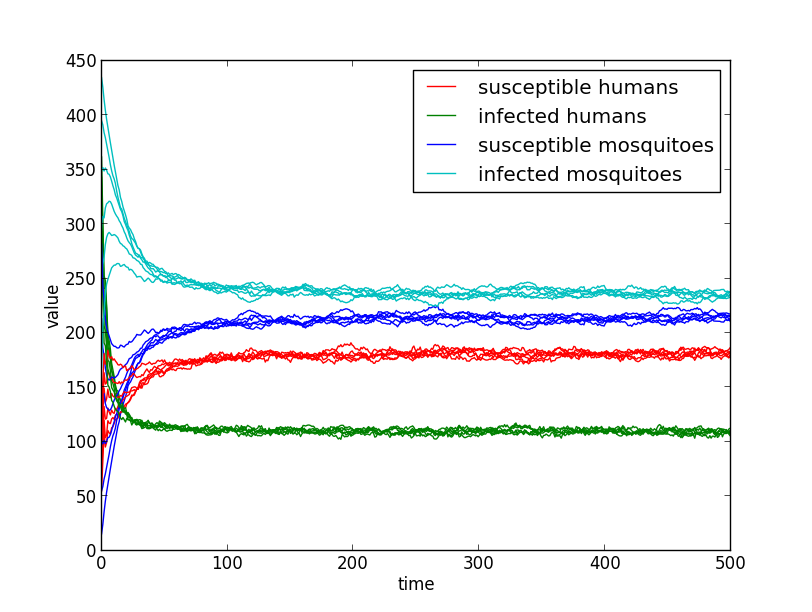
\includegraphics[scale=0.5]{var_mosquito_suscept_05_02_05_SECOND.png}
        \caption{Experimentations with 450 humans, of which 90 susceptible and 450
        mosquitoes. The amount of susceptible mosquitoes varied between 0 and
    450 }
        \label{fig:figure1}
    \end{minipage}
    \begin{minipage}[b]{0.8\linewidth}
        \centering
        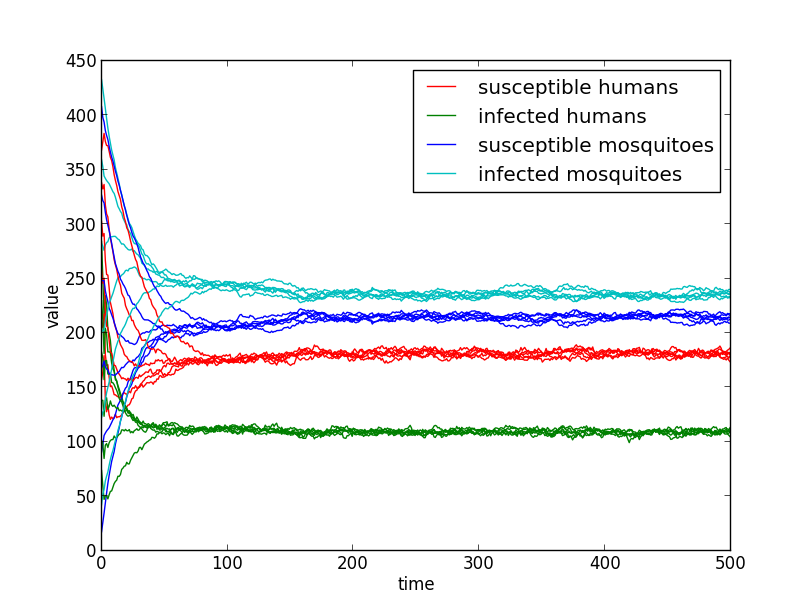
\includegraphics[scale=0.5]{var_mosquito_suscept_05_08_05_SECOND.png}
        \caption{Experimentations with 450 humans, of which 396 susceptible and 450
        mosquitoes. The amount of susceptible mosquito was varied between 0 and
        450}
        \label{fig:figure2}
    \end{minipage}
\end{figure}

\FloatBarrier
\subsection{Experimenting with other ratese}
The fact that the initial susceptibility does not seem to matter and in a matter
of 20 iteration the amount of infected mosquitoes stabilises towards a rate of
$\frac{1}{9}$th probably has to do with some of the predetermined rates. The most likely
candidates seem to be the mortality rate and immunity rate, and now will be shown if
varying the mortality rate and immunity rate increase variation in result when
choosing different susceptibility rates.

When making humans 3 times more likely to die each iteration, it does not effect
the outcome of 500 iterations at all in the case of figure
\ref{fig:death_rate} and \ref{fig:death_rate2}.
When making humans 6 times more likely to die each iteration
the same thing
happens, which doesn't encourage to variate the deathrate any more

\begin{figure}[htbp]
    \centering
    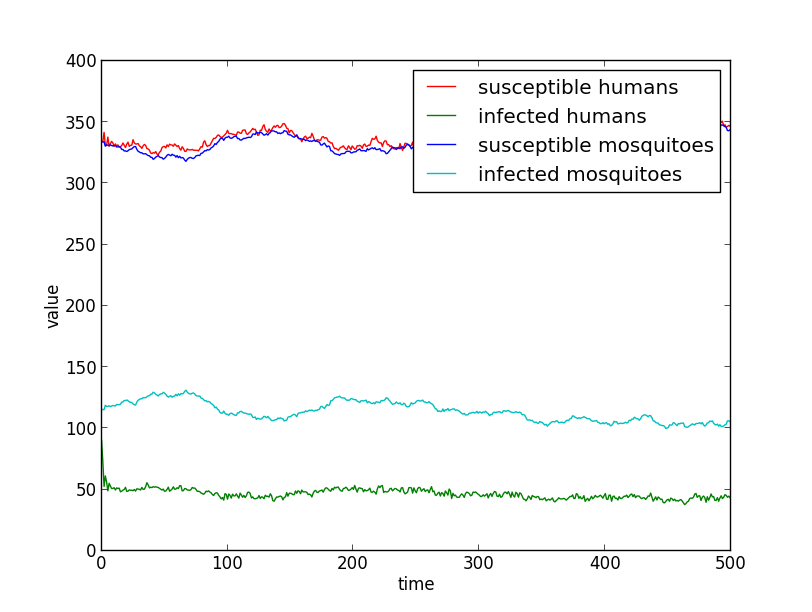
\includegraphics[width=0.7\textwidth]{05_08_05_08_higher_deathrate.png}
    \caption{3 times higher mortality rate for humans as before, with human density =
        0.5, human susceptibility = 0.8 and the same for mosquitoes
    }
    \label{fig:death_rate}
\end{figure}

\begin{figure}[htbp]
    \centering
    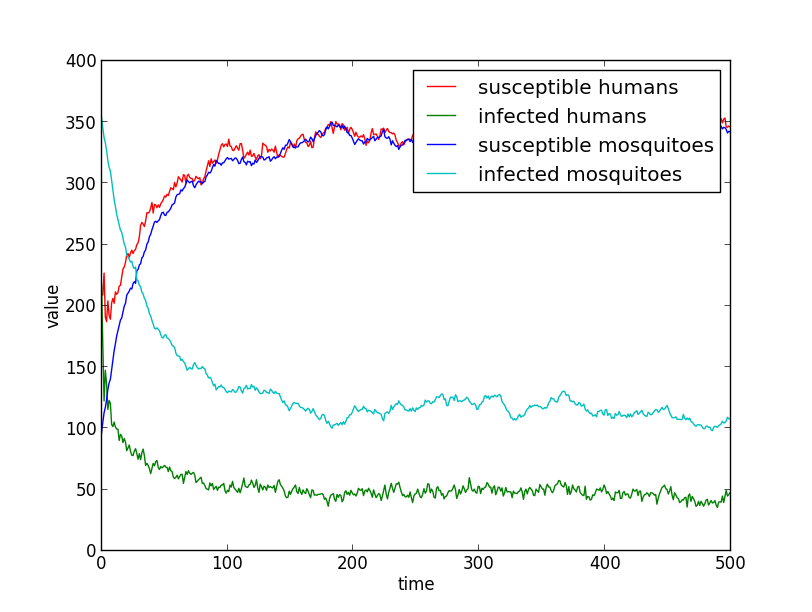
\includegraphics[width=0.7\textwidth]{05_08_05_02_higher_deathrate.png}
    \caption{3 times higher mortality rate for humans as before, with human density =
        0.5, human susceptibility is 0.8 and mosquito susceptibility is 0.2
    }
    \label{fig:death_rate2}
\end{figure}

In all the previous plots the amount of immune humans has been left out to make
the plots more coherent (and because the viewer can calculate himself the amount
of immune people using the plot at any given time), but in case of the previous
plots the immunity rate is a steady 0.11
percent. What happens if immunity is three times less likely to happen? Figure
\ref{fig:less_immunity_05_08_05_08} shows some variation from previous plots.
The amount of susceptible humansbecomes much lower as before, and the amount of
infected humans and mosquitoes by about a half higher than before. Varying the
starting susceptibility rate howerver does not give a varying outcome, as shown
in \ref{fig:less_immunity_05_08_05_02}.


\begin{figure}[htbp]
    \centering
    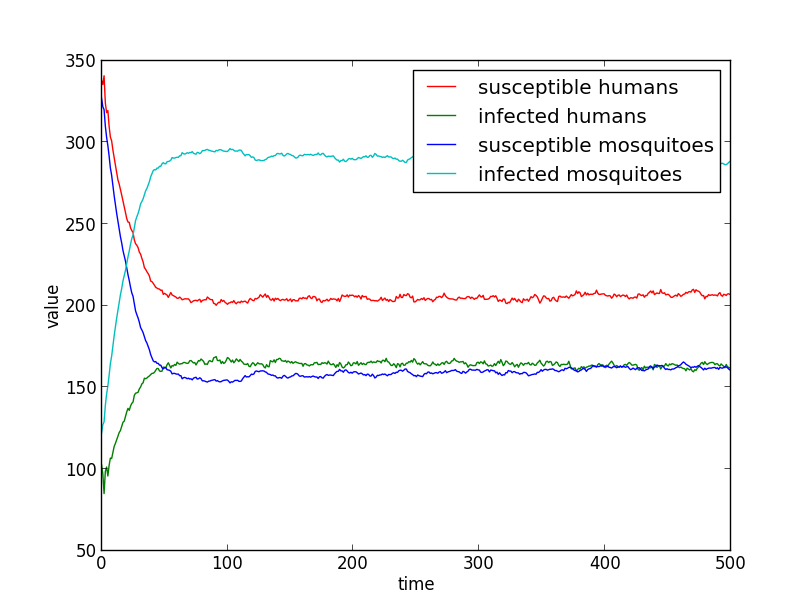
\includegraphics[width=0.9\textwidth]{less_immunity_05_08_05_08.png}
    \caption{3 times less likely immunity, with 450 humans of which 0.8
        susceptible and with 450 mosquitoes of which 0.8 susceptible.
    }
    \label{fig:less_immunity_05_08_05_08}
\end{figure}

\begin{figure}[htbp]
    \centering
    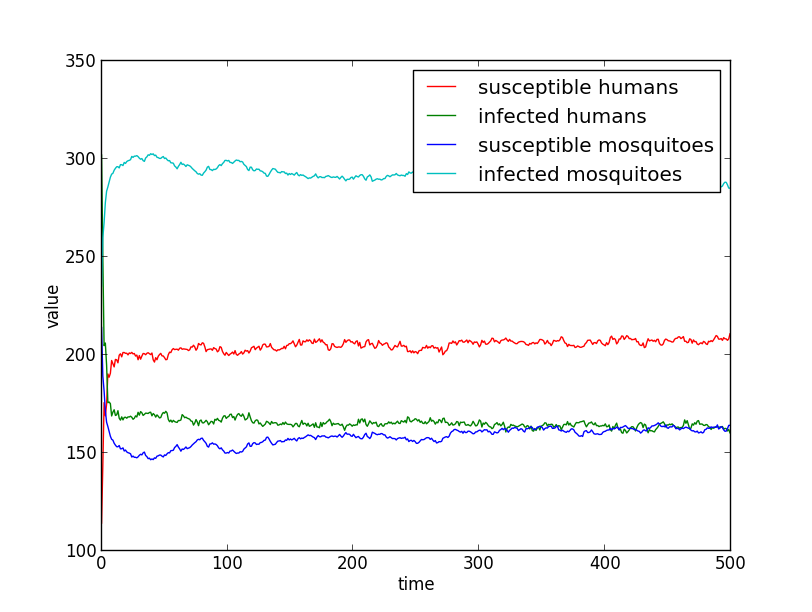
\includegraphics[width=0.9\textwidth]{less_immunity_05_08_05_02.png}
    \caption{3 times less likely immunity, with 450 humans of which 0.8
        susceptible and with 450 mosquitoes of which 0.2 susceptible.
    }
    \label{fig:less_immunity_05_08_05_02}
\end{figure}


\FloatBarrier

\section{Conclusion}
When figuring out the best conditions for malaria to be kept in existence the
ratio between humans and mosquitoes is quite important. A ration of 1 mosquito
to 1 human in this 30 $\times$ 30 grid seemed to work the best with keeping
malaria in existince. It kept the highest ratio for both infected humans as well
as for infected mosquitoes, and kept for at least 1500 iterations. It seems safe
to say that malaria wouldn't die out with these conditions, but should be
experimented with more. In case of having more mosquitoes than humans this also
has a positive effect on mosquitoes, but some extreme values should still be
tested.

The starting amount of both susceptible humans and mosquitoes can be anything
without mattering too much. At least not for the broad range of values what were
tested, but might need to be checked still for some extreme cases. The idea that
the initial susceptibility doesnt matters might seem counterintuitive as both having many susceptible mosquitoes as
well as susceptible humans would seem to mean those mosquitoes won't often
encounter an infected human, especially with the random walk that is
implemented. Although highering the mortality rate and lowering immunity 
seemed to , all of those experiments didn't confirm this intuition.

Malaria as implemented in this grid-simulation is quite a robust disease, and in
the right cases even an epidemic. Some more experimentations with elements like
moratlity rate and the immunity rate could maybe explain some of this robustness, which wasn't found with
just experimenting with the rates of density unfortunately.

% chapter malaria (end)

\end{document}
